\documentclass[11pt]{article}
\usepackage[scaled=0.92]{helvet}
\usepackage{geometry}
\geometry{letterpaper,tmargin=1in,bmargin=1in,lmargin=1in,rmargin=1in}
\usepackage[parfill]{parskip} % Activate to begin paragraphs with an empty line rather than an indent %\usepackage{graphicx}
\usepackage{amsmath,amssymb, mathrsfs,  mathtools, dsfont}
\usepackage{tabularx}
\usepackage{tikz-cd}
\usepackage[font=footnotesize,labelfont=bf]{caption}
\usepackage{graphicx}
\usepackage{xcolor}
%\usepackage[linkbordercolor ={1 1 1} ]{hyperref}
%\usepackage[sf]{titlesec}
\usepackage{natbib}
%\usepackage{tikz-cd}

\usepackage{../../Tianpei_Report}

%\usepackage{appendix}
%\usepackage{algorithm}
%\usepackage{algorithmic}

%\renewcommand{\algorithmicrequire}{\textbf{Input:}}
%\renewcommand{\algorithmicensure}{\textbf{Output:}}



\begin{document}
\title{Lecture 3: Rademacher Complexity and Vapnik-Chervonenkis Dimension}
\author{ Tianpei Xie}
\date{ Dec. 18th., 2022 }
\maketitle
\tableofcontents
\newpage
\section{PAC Learnability for Infinite Hypothese Set}
\begin{itemize}
\item \begin{remark} (\emph{\textbf{Bounding Excess Risk via Uniform Deviation}})\\
The definition of \emph{\textbf{agnostic PAC learnability}} requires that \emph{\textbf{the excess risk}} would be \underline{\emph{bounded above} \emph{\textbf{uniformly} over \textbf{all distributions}}}.
\begin{align}
L(h_n) - \inf_{h \in \cH}L(h)  &\le  2 \sup_{h\in \cH}\abs{L(h) - \widehat{L}(h)} \label{ineqn: excess_risk_bound}
\end{align} where $h^{*} = \argmin_{h\in \cH}L(h)$ and $\widehat{L}(h)$ is the training error of $g$. The second last inequality is due to the fac that $h_n$ minimizes the training error.  Thus \emph{the estimation error} can be bounded uniformly by \emph{the generalization error bound} $|L(h) - \widehat{L}(h)|$ for any $h \in \cH$.

In this chapter, we discuss various ways to bound the uniform deviation:
\begin{align*}
\sup_{h\in \cH}\abs{\widehat{L}(h) - L(h)} := \norm{\widehat{\cP}_n - \cP}{\cH}
\end{align*}
\end{remark} 

\item \begin{remark} (\emph{\textbf{Universal Consistency for Infinite Hypothesis Set}})\\
When $\abs{\cH} < \infty$, we can use sample complexity bounds that involve $\log \abs{\cH}$ for \emph{universal consistency} of ERM. Obviously, we cannod do so when $\abs{\cH} = \infty$. A general idea of analyzing infinite hypothesis set consists of \emph{\textbf{reducing the infinite case to the analysis of finite sets of hypotheses}} and then proceed as in the previous chapter. 

There are different techniques for that reduction, each relying on \emph{a different notion of \textbf{complexity}} for \emph{the family of hypotheses}. 
\end{remark}
\end{itemize}

\section{Rademacher Complexity}
\begin{itemize}
\item \begin{remark} (\emph{Notations})\\
We will continue to use $\cH$ to denote a \emph{hypothesis set} as in the previous chapters, and $h \in \cH$ an \emph{element} of $\cH$. Many of the results of this section are general and hold for an arbitrary \emph{loss function} $L: \cY \times \cY \to \bR$. To each $h: \cX \to \cY$, we can associate a function $g$:
\begin{align*}
g: (x, y) \in \cX \times \cY \to L(h(x), y)
\end{align*} without explicitly describing the specific loss $L$ used. In what follows $\cG$ will generally be interpreted as \emph{\textbf{the family of loss functions} associated to $\cH$}. 
\end{remark}


\item \begin{definition} (\emph{\textbf{Empirical Rademacher Complexity}})\\
Let $\cG$ be a family of functions mapping from $\cZ := \cX \times \cY$ to $[a, b]$ and $\cD = (z_1 \xdotx{,} z_n)$ a fixed \emph{sample} of size $n$ with elements in $\cZ$. Then, \underline{\emph{\textbf{the empirical Rademacher complexity}}} of $\cG$ \emph{with respect to the sample $\cD$} is defined as:
\begin{align}
\widehat{\mathfrak{R}}_{\cD}(\cG)&= \E{\sigma}{\sup_{g \in \cG}\frac{1}{n}\sum_{i=1}^{n}\sigma_{i}g(z_i)}   \label{eqn: rademacher_complexity}
\end{align}
where $\sigma := (\sigma_1 \xdotx{,} \sigma_n)$ are  \textbf{\emph{independent uniform random variables}} taking values in $\set{-1, +1}$. The random variables $\sigma_i$ are called \underline{\emph{\textbf{Rademacher variables}}}.
\end{definition}

\item \begin{definition}(\emph{\textbf{Rademacher Random Variable} and \textbf{Rademacher Process}})\\
\underline{\emph{A \textbf{Rademacher variables}}} is a \emph{\textbf{symmetric Bernoulli} random variable} on $\set{-1, +1}$ with \emph{equal probability} $P(\sigma_i = +1) = P(\sigma_i = -1)= \frac{1}{2}$.  \emph{A \textbf{Rademacher sequence}} $\sigma := (\sigma_1 \xdotx{,} \sigma_n)$ is seen as a \emph{uniform distribution} on binary hypercube $\set{-1, 1}^n$.

\underline{\emph{\textbf{A Rademacher process}}} indexed by the function class $\cG$ is defined as
\begin{align*}
\frR_n &:= \sum_{i=1}^n\sigma_i \delta_{g(Z_i)},
\end{align*} where $\sigma$ is a \emph{Rademacher sequence} and is independent from $Z$. It  is a \emph{\textbf{sub-gaussian} stochastic process}. $\set{\sigma_i g(Z_i)}$ \emph{\textbf{conditioning}} on $\set{Z_i}$ is a \emph{Rademacher process}.
\end{definition}

\item \begin{remark} (\emph{\textbf{How Well to Fit Random Noise}})\\
\emph{The Rademacher complexity} captures the richness of a family of functions by measuring \emph{\textbf{the degree} to which \textbf{a hypothesis set} can \textbf{fit random noise}}. The \emph{richer or more complex families} $\cH$ can generate \emph{more vectors} $h_{\cD}$ and thus \emph{better correlate with random noise}, on $\cD_n$.

The intuition is that if a hypothesis set can fit arbitrary noise, then it is too large to bound the performance of ERM, i.e. it is very likely to have overfitting (zero empirical error but arbitrary bad generalization error).
\end{remark}

\item \begin{remark}
\begin{align*}
\widehat{\mathfrak{R}}_{n}(\cG)&= \E{\sigma}{\sup_{g \in \cG}\frac{\inn{\sigma_n}{g_{n}}}{n}}
\end{align*} which measures the \emph{\textbf{correlation}} between \emph{the random noise} $\sigma_n := \set{\sigma_i}$ and $g_n \equiv  \set{g(X_i, Y_i)}_{i=1}^{n}$. The supremum $\sup_{g \in \cG} \inn{\sigma_n}{g_{n}}/n$ is a measure of how well the function class $\cH$ correlates with $\sigma$ over the sample $\cD_n$. Thus, \emph{\textbf{the empirical Rademacher complexity}} measures \emph{on average} how well \emph{\textbf{the function class}} $\cH$ \emph{\textbf{correlates with random noise}} on $\cD_n$. 
\end{remark}




\item \begin{definition} (\emph{\textbf{Rademacher Complexity}})\\
Let $\cP$ denote the distribution according to which samples are drawn. For any integer $n \ge 1$, \underline{\emph{\textbf{the Rademacher complexity}}} of $\cG$ is defined as the \emph{expectation} of \emph{the empirical
Rademacher complexity} over \emph{all samples of size $n$} drawn according to $\cP$:
\begin{align*}
\frR_{n}(\cG) &= \E{\cP^{n}}{\widehat{\mathfrak{R}}_{\cD_n}(\cG)}.
\end{align*}
\end{definition}

\item \begin{proposition} (\textbf{Uniform Bound via Rademacher Complexity}) \citep{mohri2018foundations}\\
Let $\cG$ be a family of functions mapping from $\cZ$ to $[0, 1]$. Then, for any $\delta > 0$, \textbf{with probability at least} $1 - \delta$, each of the following holds for all $g \in \cG$:
\begin{align}
\E{}{g(Z)} &\le \frac{1}{n}\sum_{i=1}^{n}g(Z_i) + 2 \frR_{n}(\cG)  + \sqrt{\frac{\log(1 / \delta)}{2n}} \label{eqn: Rademacher_bound_1}
\end{align}
and
\begin{align}
\E{}{g(Z)} &\le \frac{1}{n}\sum_{i=1}^{n}g(Z_i) + 2 \widehat{\mathfrak{R}}_{n}(\cG) + 3\sqrt{\frac{\log(2 / \delta)}{2n}} \label{eqn: Rademacher_bound_2}
\end{align}
\end{proposition}

\item \begin{proof}
Define a function $\Phi$ on $\cD_n$ by
\begin{align*}
\Phi(\cD_n) &:= \sup_{g \in \cG}\brac{\frac{1}{n}\sum_{i=1}^{n}g(Z_i) - \E{}{g(Z)}}.
\end{align*} This function has \emph{bounded difference} if \emph{only one sample makes changes}. In particular, let $\cD_n \equiv (Z_1 \xdotx{,} Z_n)$ and $\widetilde{\cD}_n^{(i)} \equiv (Z_1 \xdotx{,} Z_{i-1}, Z_i', Z_{i+1} \xdotx{,} Z_n)$. Then
\begin{align*}
\abs{\Phi(\cD_n) - \Phi(\widetilde{\cD}_n^{(i)})} &\le \frac{1}{n}\sup_{g \in \cG}\abs{g(Z_i) - g(Z_i')} \le \frac{1}{n}.
\end{align*}
%Note that $\Phi(\cD_n)$ is a \emph{random variable} taking values in $[-1, 1]$. 
The proof consists of three parts:
\begin{enumerate}
\item Bound \emph{the probability} of \emph{\textbf{tail event of $\Phi$}} 
\begin{align*}
\Phi(\cD_n) - \E{\cP^{n}}{\Phi(\cD_n)}
\end{align*} This part follows from \emph{the bounded difference inequality}: for any $\delta > 0$, with probability at least $1 - \delta/2$, 
\begin{align}
\Phi(\cD_n) - \E{\cP^{n}}{\Phi(\cD_n)} \le \sqrt{\frac{\log(2/\delta)}{2n}} \label{pf: rad_comp_bound_1}
\end{align}


\item Bound the \emph{expectation} $\E{\cP^{n}}{\Phi(\cD_n)}$ by \emph{Rademacher complexity on $\cG$}
\begin{align*}
\E{\cP^{n}}{\Phi(\cD_n)} &\le 2   \frR_{n}(\cG).
\end{align*} Recall that $Z'  = (Z_1 \xdotx{,} Z_{i-1}, Z_i', Z_{i+1} \xdotx{,} Z_n)$ and $Z = (Z_1 \xdotx{,} Z_n)$. We know that $\E{Z'}{\frac{1}{n}\sum_{i=1}^{n}g(Z_i')} =  \E{}{g(Z)}$ since $Z'$ and $Z$ are independent identically distributed.
\begin{align}
\E{\cP^{n}}{\Phi(\cD_n)} &= \E{Z}{\sup_{g \in \cG}\brac{\frac{1}{n}\sum_{i=1}^{n}g(Z_i) - \E{}{g(Z)}}} \nonumber\\
&= \E{Z}{\sup_{g \in \cG}\E{Z'}{ \frac{1}{n}\sum_{i=1}^{n}g(Z_i) - \frac{1}{n}\sum_{i=1}^{n}g(Z_i') }} \nonumber\\
& \;\;(\text{Jenson's inequality and convexity of $\sup$}) \nonumber\\
&\le \E{Z, Z'}{\sup_{g \in \cG}\brac{ \frac{1}{n}\sum_{i=1}^{n}g(Z_i) - \frac{1}{n}\sum_{i=1}^{n}g(Z_i') }} \nonumber\\
& \;\; (\text{symmetrization}) \nonumber\\
& =\E{Z, Z', \sigma}{\sup_{g \in \cG}\brac{\frac{1}{n}\sum_{i=1}^{n}\sigma_i\paren{g(Z_i) - g(Z_i')}}} \nonumber\\
& \;\; (\text{sub-additivy of $\sup$}) \nonumber\\
&\le \E{Z, \sigma}{\sup_{g \in \cG}\brac{\frac{1}{n}\sum_{i=1}^{n}\sigma_i g(Z_i) }}+ \E{Z', \sigma}{\sup_{g \in \cG}\brac{\frac{1}{n}\sum_{i=1}^{n}-\sigma_i g(Z_i')}} \nonumber\\
&= 2 \E{Z, \sigma}{\sup_{g \in \cG}\brac{\frac{1}{n}\sum_{i=1}^{n}\sigma_i g(Z_i) }} := 2\frR_n(\cG) \label{pf: rad_comp_bound_2}
\end{align}
The \emph{\textbf{symmetrization step}} works since $\sigma_i = \pm 1$ with equal probability. If $\sigma_i = +1$, then the summand is unchanged. If $\sigma_i = -1$, the summand is swapped but the distribution  is unchanged as well since  $Z'$ and $Z$ are independent identically distributed.
The last equality follows from the definition of Rademacher complexity and the fact that $\sigma_i$ and $-\sigma_i$ follow the same distribution since they are symmetric Bernoulli random variables. Finally, replacing $\E{\cP^{n}}{\Phi(\cD_n)}$ by its upper bound $2\frR_n(\cG)$ and $\delta/2 \to \delta$ gives us  inequality \eqref{eqn: Rademacher_bound_1}.

\item Bound \emph{the probability} of \emph{tail events} for \emph{empircal Rademacher complexity}:
\begin{align*}
\frR_{n}(\cG)  - \widehat{\mathfrak{R}}_{n}(\cG)
\end{align*} In this part, we use \emph{the bounded difference inequality} again, noticing that \emph{the empirical Rademacher complexity} is function with bounded difference $1/n$. Therefore, 
\begin{align}
\frR_{n}(\cG)  &\le \widehat{\mathfrak{R}}_{n}(\cG) + \sqrt{\frac{\log(2/\delta)}{2n}} \label{pf: rad_comp_bound_3}
\end{align}
Finally, we combines the inequalities in \eqref{eqn: Rademacher_bound_1} and \eqref{pf: rad_comp_bound_3} using union bounds to obtain the final result. \qed
\end{enumerate}
\end{proof} 

\item \begin{remark}(\textbf{\emph{Rademacher Complexity as Uniform Bound}}) \\
The above proposition states that any positive integer $n \ge 1$ and any scalar $\delta \ge 0$, with probability at least $1 - \delta$, we have
\begin{align*}
\sup_{g \in \cG}\abs{\frac{1}{n}\sum_{i=1}^{n}g(Z_i)  - \E{}{g(Z)}} \le 2 \frR_{n}(\cG)  + \sqrt{\frac{\log(1 / \delta)}{2n}}
\end{align*}
\end{remark}

\item \begin{remark}(\textbf{\emph{Symmetrization}}) \\
The techinque that develops the uniform deviation bound via \emph{Rademacher complexity} is called \emph{\textbf{symmetrization}}. Consider \emph{\textbf{the empirical process}}
\begin{align*}
g \to \paren{\widehat{\cP}_n - \cP}g = \frac{1}{n}\sum_{i=1}^{n}(g(Z_i)  - \cP g)
\end{align*} where $\cP g := \int g d\cP = \E{\cP}{g(Z)}$ is seen as an \emph{operator} on function (by identification of the measure and functional). The \emph{symmetrization} refer to the idea to replace \emph{the empirical process} with \emph{\textbf{a symmetrized process}}
\begin{align*}
g \to \widehat{\cP}_n^{\epsilon}g := \frac{1}{n}\sum_{i=1}^{n}\epsilon_i g(Z_i)
\end{align*} where $\epsilon := (\epsilon_1 \xdotx{,} \epsilon_n)$ are \emph{\textbf{i.i.d. Rademacher random variables}} (symmetric Bernoulli random variable on $\set{-1, 1}$) and they are  \emph{\textbf{independent}} of $(Z_1 \xdotx{,} Z_n)$. The idea is that, for fixed $(Z_1 \xdotx{,} Z_n)$, the symmetrized empirical measure is a \emph{Rademacher process}, hence a \emph{sub-Gaussian process}.

\begin{lemma} (\textbf{Symmetrization}). \citep{wellner2013weak}\\
For every \textbf{nondecreasing}, \textbf{convex} $\Phi: \bR \to \bR$ and class of measurable functions $\cG$,
\begin{align*}
\E{}{\Phi\paren{\norm{\widehat{\cP}_n - \cP}{\cG}}} &\le \E{}{\Phi\paren{2\norm{\widehat{\cP}_n^{\epsilon}}{\cG}}}
\end{align*}
\end{lemma}

\end{remark}

\item \begin{lemma} (\textbf{Rademacher Complexity for 0-1 Loss}) \citep{mohri2018foundations}\\
Let $\cH$ be a family of functions taking values in $\{-1, +1\}$ and let $\cG$ be the family of loss functions associated to $\cH$ for \textbf{the zero-one loss}: 
\begin{align*}
\cG := \set{(x,y) \mapsto \mathds{1}_{h(x) \neq y}:  h \in \cH}.
\end{align*}
For any sample $\cD = ((X_1, Y_1) \xdotx{,} (X_n, Y_n))$ of elements in $\cX \times \{-1, +1\}$, let $\cD_{\cX} := (X_1 \xdotx{,} X_n)$. Then, the following relation holds between \textbf{the empirical Rademacher complexities} of $\cG$ and $\cH$:
\begin{align*}
\widehat{\frR}_{\cD}(\cG) &\le \frac{1}{2}\widehat{\frR}_{\cD_{\cX}}(\cH)
\end{align*} This implies that $\frR(\cG) = \frac{1}{2}\frR(\cH)$. 
\end{lemma} (Hint: $ \mathds{1}_{h(x) \neq y} := \frac{1}{2}(1 - y h(x))$. Also $\sigma$ and $-\sigma y$ have the same distribution.)

\item This immediately gives us the result below:
\begin{proposition} \label{prop: generalization_bound_Rademacher} (\textbf{Rademacher Complexity Bound for Binary Classification})\citep{mohri2018foundations}\\
Let $\cH$ be a family of functions taking values in $\{-1, +1\}$  and let $\cP$ be the distribution over the input space $\cX$. Then, for any $\delta > 0$, \textbf{with probability at least} $1 - \delta$ over a sample $\cD_{n}$ of size $n$ drawn according to $\cP_{X}$, each of the following holds for \textbf{any} $h \in \cH$:
\begin{align}
L(h) &\le \widehat{L}_{n}(h) + \frR_{n}(\cH) + \sqrt{\frac{\log(1 / \delta)}{2n}}  \label{eqn: Rademacher_binary_loss_bound_1}
\end{align} and
\begin{align}
L(h) &\le \widehat{L}_{n}(h) + \widehat{\frR}_{n}(\cH) +  3\sqrt{\frac{\log(2 / \delta)}{2n}}.  \label{eqn: Rademacher_binary_loss_bound_2}
\end{align}
\end{proposition}

\item \begin{remark} (\emph{\textbf{Compute Empirical Rademacher Complexity}})\\
Note that the \emph{Rademacher variable} $\sigma_i$ and $-\sigma_i$ have the same distribution. So
\begin{align*}
\widehat{\frR}_{\cD}(\cH)&= \E{\sigma}{\sup_{h \in \cH}\frac{1}{n}\sum_{i=1}^{n}(-\sigma_{i}h(X_i))} = -\E{\sigma}{\inf_{h \in \cH}\frac{1}{n}\sum_{i=1}^{n}\sigma_{i}h(X_i)}
\end{align*} Now, for \emph{a fixed value of $\sigma$}, computing 
\begin{align*}
\inf_{h \in \cH}\frac{1}{n}\sum_{i=1}^{n}\sigma_{i}h(X_i)
\end{align*} is equivalent to an \emph{\textbf{empirical risk minimization problem}}, which is known to be \emph{\textbf{computationally hard}} for some hypothesis sets. Thus, in some cases, computing $\widehat{\frR}_{\cD}(\cH)$ could be computationally hard. 
\end{remark}

\item \begin{proposition}(\textbf{Talagrand's Contraction Principle}) \citep{boucheron2013concentration, vershynin2018high}\\
Let $x_1 \xdotx{,} x_n$ be vectors whose real-valued components are indexed by $T$, that is, $x_i = (x_{i,s})_{s \in T}$. For each $i = 1 \xdotx{,} n$, let $\varphi_i : \bR \to \bR$ be a \textbf{$1$-Lipschitz function} such that $\varphi_i(0) = 0$. Let $\epsilon_1 \xdotx{,} \epsilon_n$ be independent Rademacher random variables, and let $\Psi: [0, \infty) \to \bR$ be a \textbf{non-decreasing convex} function.  Then
\begin{align}
\E{}{\Psi\paren{\sup_{s\in T}\sum_{i=1}^n \epsilon_i \varphi_i(x_{i,s})}} \le \E{}{\Psi\paren{\sup_{s\in T}\sum_{i=1}^n \epsilon_i  x_{i,s}}}\label{ineqn: contraction_principle_1}
\end{align} and
\begin{align}
\E{}{\Psi\paren{\frac{1}{2}\sup_{s\in T}\abs{\sum_{i=1}^n \epsilon_i \varphi_i(x_{i,s})}}} \le \E{}{\Psi\paren{\sup_{s\in T}\abs{\sum_{i=1}^n \epsilon_i  x_{i,s}}}}.\label{ineqn: contraction_principle_2}
\end{align}
\end{proposition}

The proof of this result need  the following lemma
\begin{lemma}\citep{boucheron2013concentration, vershynin2018high}\\
Let $\Psi : \bR\to \bR$ denote a \textbf{convex non-decreasing function}. Let $\varphi: \bR \to \bR$ be a $1$-Lipschitz function such that $\varphi_i(0) = 0$. Let $T \subset \bR^2$. Then
\begin{align*}
\Psi\paren{\sup_{s \in T}\set{s_1 + \varphi(s_2)}} + \Psi\paren{\sup_{s \in T}\set{s_1 - \varphi(s_2)}} &\le \Psi\paren{\sup_{s \in T}\set{s_1 + s_2}} + \Psi\paren{\sup_{s \in T}\set{s_1 - s_2}}
\end{align*}
\end{lemma}

\item \begin{corollary} (\textbf{Talagrand's Lemma}) \citep{mohri2018foundations}\\
Let $\varphi: \bR \to \bR$ be an $L$-Lipschitz. Then, for any hypothesis set $\cH$ of real-valued functions, the following inequality holds:
\begin{align}
\widehat{\frR}_{\cD}(\varphi \circ \cH)  \le L\, \widehat{\frR}_{\cD}(\cH) \label{ineqn: rademacher_complexity_contraction}
\end{align}
\end{corollary}

\item \begin{proposition}(\textbf{Rademacher Complexity of a Convex Hull of Function Class}\\
Let $\cH$ be a set of functions mapping from $\cX$ to $\bR$. Then, for any sample $\cD$, we have
\begin{align}
\widehat{\frR}_{\cD}(\text{conv}(\cH))  = \widehat{\frR}_{\cD}(\cH) \label{eqn: rademacher_complexity_convex_hull}
\end{align} where $\text{conv}(\cH)$ is \textbf{the convex hull} of set $\cH$
\begin{align*}
\text{conv}(\cH) := \set{\sum_{k=1}^{p}\lambda_k h_k:  p \ge 1, \forall k \in [1, p], \lambda_k \ge 0, h_k \in \cH, \sum_{k=1}^{p}\lambda_k \le 1}.
\end{align*}
\end{proposition}
\begin{proof}
\begin{align*}
\widehat{\frR}_{\cD}(\text{conv}(\cH))  &= \E{\sigma}{\sup_{g \in \text{conv}(\cH)}\frac{1}{n}\sum_{i=1}^{n}\sigma_i g(X_i) }\\
&= \frac{1}{n}\E{\sigma}{\sup_{h_{1} \xdotx{,} h_{p} \in \cH}\;\sup_{ \set{\lambda_k} \in \Delta_{p} }\sum_{i=1}^{n}\sigma_i \sum_{k=1}^{p}\lambda_k h_{k}(X_i)}\\
&= \frac{1}{n}\E{\sigma}{\sup_{h_{1} \xdotx{,} h_{p} \in \cH}\;\sup_{ \set{\lambda_k} \in \Delta_{p} }\sum_{k=1}^{p}\lambda_k\sum_{i=1}^{n}\sigma_i  h_{k}(X_i)}
\end{align*} Note that extreme point of a convex hull is its vertex, so the supremum of $\sum_{k=1}^{p}\lambda_k (\sum_{i=1}^{n}\sigma_i  h_k(X_i))$ over $\lambda$ can only be reached at one of $\set{\sum_{i=1}^{n}\sigma_i  h_{k}(X_i)}_{k=1}^{p}$. Thus above equality becomes
\begin{align*}
\widehat{\frR}_{\cD}(\text{conv}(\cH))  &= \frac{1}{n}\E{\sigma}{\sup_{h_{1} \xdotx{,} h_{p} \in \cH}\max_{k \in [1,p]}\sum_{i=1}^{n}\sigma_i  h_{k}(X_i)}\\
&= \frac{1}{n}\E{\sigma}{\sup_{h \in \cH}\sum_{i=1}^{n}\sigma_i  h(X_i)} = \widehat{\frR}_{\cD}(\cH). \qed
\end{align*}
\end{proof}
\end{itemize}

\section{Vapnik-Chervonenkis Dimension}
\subsection{Definition of Vapnik-Chervonenkis Dimension}
\begin{itemize}
%\item \begin{remark}
%%Recall the decomposition of generalization error:
%%\begin{align*}
%%L(g_n^{*}) - L^{*} &=\underbrace{\paren{L(g_n^{*}) - \inf_{g \in \cH}L(g)}}_{\text{\emph{estimation error}}} + \underbrace{\paren{\inf_{g \in \cH}L(g) - L^{*}}}_{\text{\emph{approximation error}}}.
%%\end{align*} 
%%where the first term is called \emph{estimation error} and the second term is called approximation error.  
%The definition of \emph{\textbf{PAC learnability}} requires that \emph{the estimation error} would be bounded \emph{\textbf{uniformly} over \textbf{all distributions}}.
%Can \emph{infinite-size classes} be learnable, and, if so, what determines their \emph{sample complexity} ?
%\end{remark}
\item \begin{remark} (\emph{\textbf{Restriction based on Behavior of Functions on Data $\cD$}})\\
Recall the No-Free-Lunch theorem and its proof \citep{shalev2014understanding}. There, we have shown that \emph{without restricting the hypothesis class}, for any learning algorithm, \emph{an adversary can construct a distribution} for which \emph{the learning algorithm will perform poorly}, while there is \emph{another learning algorithm that will succeed on the same distribution}. To do so, the adversary used a finite set $\cD \subset \cX$ and considered a family of distributions that are
\emph{\textbf{concentrated on elements of $\cD$}}. Each distribution was \emph{derived from a ``true" target function} from $\cD$ to $\set{0,1}$. To make any algorithm fail, the adversary used the power of choosing a target function from the set of \emph{all possible functions} from $\cD$ to $\set{0,1}$.

When considering \emph{PAC learnability of a hypothesis class $\cH$}, the adversary is restricted to \emph{constructing distributions} for which \emph{some hypothesis $h \in \cH$ achieves a zero risk}. Since we are considering \emph{\textbf{distributions that are concentrated on elements of $\cD$}}, we should study how $\cH$ behaves on $\cD$
\end{remark}

\item \begin{definition} (\emph{\textbf{Restriction of $\cH$ to $\cD$}}). \\
Let $\cH$ be a class of functions from $\cX$ to $\set{0,1}$ and let $\cD = \set{x_1 \xdotx{,} x_n} \subset \cX$. 

\underline{\emph{\textbf{The restriction of $\cH$ to $\cD$}}} is \emph{the set of functions} from $\cD$ to $\set{0,1}$ that can be \emph{derived from} $\cH$. That is,
\begin{align*}
\cH_{\cD} := \set{(h(x_1) \xdotx{,} h(x_n)): h \in \cH},
\end{align*}
where we \emph{\textbf{represent}} each function from $\cX$ to $\set{0,1}$ as a \emph{\textbf{vector}} in $\set{0,1}^{\abs{\cD}}$.
\end{definition}

\item \begin{remark} (\textbf{\emph{What You See Is All You Know}})\\
Using the output of functions on \emph{\textbf{a finite set of samples}}, we can define an \emph{\textbf{equivalence relationship}}: $f \sim g$ if and only if their \emph{\textbf{outputs}} vector on given finite set $\cD_m$ are \emph{\textbf{the same}}. Thus, unlike the original space $\cH$, \emph{\textbf{the quotient space}} $\cH/\sim$ is a much \emph{simpler function space} with \emph{\textbf{finite dimensional representation}}. 

In other word, \underline{\emph{\textbf{what you see is all you know}}}, i.e. there is no way to distinguish $f$ and $g$ beyond their answers to given limited set of questions in $\cD$.

%One can also think of this in functional analysis, where a set of $m$ evaluation functional $\delta_{x_i}(f) = f(x_i), 1\le i\le m$ are given and the function space is reparameterized using these $m$ functionals. 
\end{remark}

\item \begin{definition}(\emph{\textbf{Shattering}}). \\
A hypothesis class $\cH$ \underline{\emph{\textbf{shatters}} a finite set $\cD \subset \cX$} if \emph{\textbf{the restriction of $\cH$ to $\cD$}} is the set of \emph{\textbf{all functions}} from $\cD$ to $\set{0,1}$. That is, 
\begin{align*}
\abs{\cH_{\cD}} &= 2^{\abs{\cD}}.
\end{align*}
\end{definition}

\item \begin{remark}
Whenever some set $\cD$ is \emph{\textbf{shattered}} by $\cH$, the \emph{\textbf{adversary}} is \emph{\textbf{not restricted} by $\cH$}, as they can \emph{\textbf{construct a distribution over $\cD$}} based on \emph{\textbf{any}} target function from $\cD$ to $\set{0,1}$, while still maintaining the realizability assumption. 
\end{remark}

\item The following is the corollary of \emph{the No Free Lunch Theorem}:
\begin{corollary} \citep{shalev2014understanding}\\
Let $\cH$ be a hypothesis class of functions from $\cX$ to $\set{0,1}$. Let $n$ be a training set size. Assume that there exists a set $\cD \subset X$ of size $2n$ that is \textbf{shattered} by $\cH$. Then, for any learning algorithm, $\cA$, there exist a \textbf{distribution} $\cP$ over $\cX \times \set{0,1}$
and a predictor $h \in \cH$ such that 
\begin{align*}
L_{\cP}(h) = 0
\end{align*}
but \textbf{with probability of at least} $1/7$ over the choice of $\cD \sim \cP^n$ we have that 
\begin{align*}
L_{\cP}(\cA(\cD)) \ge 1/8.
\end{align*}
\end{corollary}

\item \begin{remark} (\emph{\textbf{A Model that can Explain Everything is Worthless}})\\
If $\cH$ \emph{\textbf{shatters}} some set $\cD$ of size $2m$ then we cannot learn $\cH$ using $m$ examples. 

Intuitively, if a set $\cD$ is \emph{\textbf{shattered}} by $\cH$, and we receive a sample containing half the instances of $\cD$, the labels of these instances give us \emph{\textbf{no information} about the labels of the \textbf{rest} of the instances} in $\cD$ - \emph{\textbf{every possible labeling of the rest of the instances can be explained by some hypothesis in $\cH$}}. 

Philosophically,

\underline{\emph{\textbf{If someone can explain every phenomenon, his explanations are worthless}}}.
\end{remark}

\item \begin{definition} (\emph{\textbf{VC-Dimension}}). \\
\underline{\emph{\textbf{The Vapnik-Chervonenkis (VC) dimension}}} of a hypothesis class $\cH$, denoted $VCdim(\cH)$ or simply $v(\cH)$, is \emph{\textbf{the \underline{maximal size}} of a set $\cD \subset \cX$ that can be \textbf{shattered} by $\cH$}.

If $\cH$ can shatter sets of \emph{\textbf{arbitrarily large size}} we say that $\cH$ has \underline{\emph{\textbf{infinite VC-dimension}}}.
\end{definition}

\item \begin{theorem} (\textbf{No Free Lunch, VC Dimension}) \citep{shalev2014understanding}\\
Let $\cH$ be a class of \textbf{infinite VC-dimension}. Then, $\cH$ is \textbf{not PAC learnable}.
\end{theorem}

\end{itemize}

\subsection{Growth Function}
\begin{itemize}
\item \begin{remark}
We defined the notion of \emph{\textbf{shattering}}, by considering \emph{\textbf{the restriction of $\cH$} to a finite set of instances}. The \emph{growth function} measures the \emph{maximal ``\textbf{effective}" size of $\cH$ on a set of $n$ examples}. Formally:
\end{remark}

\item \begin{definition} (\emph{\textbf{Growth Function}}). \\
Let $\cH$ be a hypothesis class. Then \underline{\emph{\textbf{the growth function of $\cH$}}}, denoted $\tau_{\cH}: \bN \to \cN$, is defined as
\begin{align*}
\tau_{\cH}(n) &:= \max_{\cD \subset \cX: \abs{\cD} = n}\abs{\cH_{\cD}}.
\end{align*}
In words, $\tau_{\cH}(n)$ is \textbf{\emph{the number of different functions}} from a set $\cD$ of \emph{\textbf{size $n$}} to $\set{0,1}$ that can be obtained by \emph{\textbf{restricting $\cH$ to $\cD$}}.
\end{definition}

\item \begin{remark}
if $VCdim(\cH) = d$ then for any $n \le d$ we have $\tau_{\cH}(n) = 2^n$. In such cases, $\cH$ induces \emph{all possible functions from} $\cD$ to $\set{0,1}$. 
\end{remark}

\item \begin{lemma} (\textbf{Sauer's Lemma}). \citep{shalev2014understanding, mohri2018foundations}\\
Let $\cH$ be a hypothesis class with $VCdim(\cH) \le d < \infty$. Then, for all $n$, 
\begin{align}
\tau_{\cH}(n) &\le \sum_{i=0}^{d}{{n}\choose{i}} \label{eqn: sauer_lemma_1}
\end{align}
In particular, if $n > d + 1$ then
\begin{align}
\tau_{\cH}(n) &\le \paren{\frac{en}{d}}^{d}. \label{eqn: sauer_lemma_2}
\end{align}
\end{lemma}
\begin{proof}
To prove the lemma it suffices to prove the following \emph{stronger claim}: For any $\cD = \set{x_1 \xdotx{,} x_n}$ we have
\begin{align}
\forall\, \cH, \; \abs{\cH_{\cD}} \le  \abs{\set{\cB \subseteq \cD: \cH\text{ shatters }\cB}}\label{eqn: sauer_lemma_3}
\end{align} The reason why Equation \eqref{eqn: sauer_lemma_3} is sufficient to prove the lemma is that if
$VCdim(\cH) \le d$ then no set whose size is \emph{larger than} $d$ is \emph{shattered} by $\cH$ and therefore
\begin{align*}
\abs{\set{\cB \subseteq \cD: \cH\text{ shatters }\cB}} \le  \sum_{i=0}^{d}{{n}\choose{i}}.
\end{align*}
When $n > d + 1$ the right-hand side of the preceding is \emph{at most} $\paren{\frac{en}{d}}^{d}$ since
\begin{align*}
 \sum_{i=0}^{d}{{n}\choose{i}}1^{d- i} &\le  \sum_{i=0}^{d}{{n}\choose{i}}\paren{\frac{n}{d}}^{d - i}\\
 &\le  \sum_{i=0}^{n}{{n}\choose{i}}\paren{\frac{n}{d}}^{d - i} \\
 &= \paren{\frac{n}{d}}^{d} \sum_{i=0}^{n}{{n}\choose{i}}\paren{\frac{d}{n}}^{i} \\
 &= \paren{\frac{n}{d}}^{d}\paren{1 + \frac{d}{n}}^n \le \paren{\frac{n}{d}}^{d}e^{d}
\end{align*} where $1+x \le e^x$.



We are left with proving Equation \eqref{eqn: sauer_lemma_3} and we do it using an \emph{\textbf{inductive argument}}. 
\begin{enumerate}
\item For $n = 1$, no matter what $\cH$ is, either both sides of Equation \eqref{eqn: sauer_lemma_3} equal $1$ or both sides equal $2$ (\emph{the empty set} is always considered to be shattered by $\cH$).

\item  \emph{Assume} Equation \eqref{eqn: sauer_lemma_3} holds for sets of size $k < n$ and let us prove it for sets of size $n$. 
Fix $\cH$ and $\cD = \set{x_1 \xdotx{,} x_n}$. Denote $\cD_{-1} = \set{x_2 \xdotx{,} x_n}$ and in addition, define the
following two sets:
\begin{align*}
Y_{0} = \set{(y_2 \xdotx{,} y_n): (0, y_2 \xdotx{,} y_n) \in \cH_{\cD} \lor  (1, y_2 \xdotx{,} y_n) \in \cH_{\cD}},
\end{align*}
and
\begin{align*}
Y_{1} = \set{(y_2 \xdotx{,} y_n): (0, y_2 \xdotx{,} y_n) \in \cH_{\cD} \land  (1, y_2 \xdotx{,} y_n) \in \cH_{\cD}}.
\end{align*}
It is easy to verify that $\abs{\cH_{\cD}} = \abs{Y_0} + \abs{Y_1}$ (See Figure \ref{fig: proof_sauer_lemma}). Additionally, since $Y_0 = \cH_{\cD_{-1}}$, using \emph{the induction assumption} (applied on $\cH$ and $\cD_{-1}$) we have that
\begin{align*}
\abs{Y_0} = \abs{\cH_{\cD_{-1}}} &\le \abs{\set{\cB \subseteq \cD_{-1}: \cH\text{ shatters }\cB}} \\
&=  \abs{\set{\cB \subseteq \cD: x_1 \not\in \cB \land \cH\text{ shatters }\cB}}.
\end{align*}
Next, define $\cH' \subseteq \cH$ to be
\begin{align*}
\cH'  &= \set{h \in \cH : \exists\,h' \in \cH\text{ s.t. }(1 - h'(x_1), h'(x_2) \xdotx{,} h'(x_n)) = (h(x_1), h(x_2)  \xdotx{,} h(x_n)) },
\end{align*}
namely, $\cH'$ contains pairs of hypotheses $(h, h')$ that \emph{agree on $\cD_{-1}$ and differ on $x_1$}. Using this definition, it is clear that if $\cH'$ \emph{shatters} a set $\cB \subseteq \cD$ then it \emph{also shatters} the set $\cB \cup \set{x_1}$ and \emph{vice versa}. 

\begin{figure}
\begin{minipage}[t]{1\linewidth}
  \centering
  \centerline{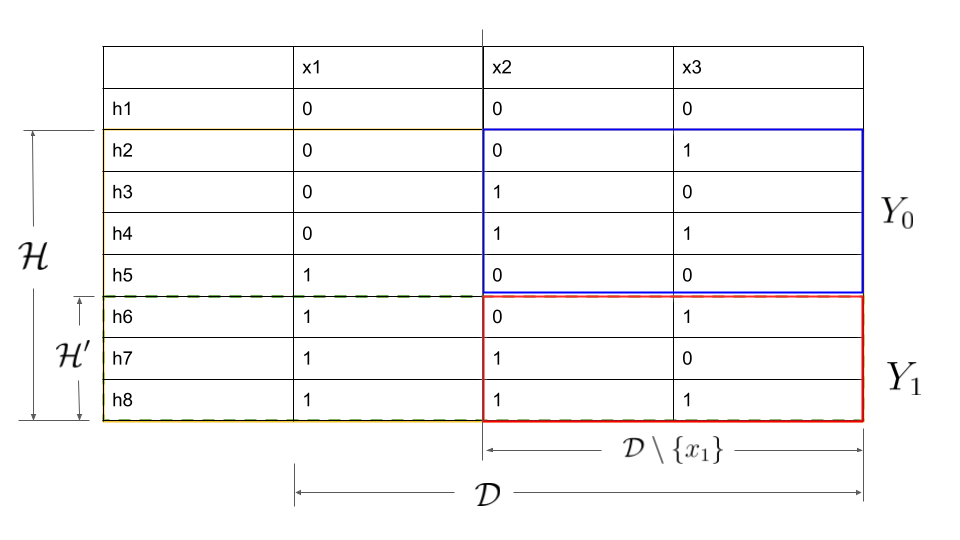
\includegraphics[scale = 0.4]{proof_sauer_lemma.png}}
\end{minipage}
\caption{\footnotesize{\textbf{Proof of Sauer's lemma. $Y_0 = \cH_{\cD\setminus \set{x_1}}$ (blue) and $Y_1 = \cH'_{\cD\setminus \set{x_1}}$ (red) where $\cH'$ are hypotheses $h'\in \cH$ so that there exists $h\in \cH$ with opposite labeling at $x_1$.   \citep{shalev2014understanding}}}}
\label{fig: proof_sauer_lemma}
\end{figure}

Combining this with the fact that $Y_1 = \cH'_{\cD_{-1}}$ and using the inductive assumption (now applied on $\cH'$ and $\cD_{-1}$ ) we obtain that
\begin{align*}
\abs{Y_1} = \abs{ \cH'_{\cD_{-1}}} &\le \abs{\set{\cB \subseteq \cD_{-1}:  \cH'\text{ shatters }\cB }} \\
&= \abs{\set{\cB \subseteq \cD_{-1}:  \cH'\text{ shatters }\cB\cup\set{x_1} }} \\
&= \abs{\set{\cB \subseteq \cD:  x_1 \in \cB \land \cH'\text{ shatters }\cB }} \\
&= \abs{\set{\cB \subseteq \cD:  x_1 \in \cB \land \cH \text{ shatters }\cB }}.
\end{align*}
Overall, we have shown that
\begin{align*}
\abs{\cH_{\cD}} &= \abs{Y_0} + \abs{Y_1} \\
&\le \abs{\set{\cB \subseteq \cD: x_1 \not\in \cB \land \cH\text{ shatters }\cB}} +  \abs{\set{\cB \subseteq \cD:  x_1 \in \cB \land \cH \text{ shatters }\cB }}\\
&= \abs{\set{\cB \subseteq \cD: \cH\text{ shatters }\cB}}
\end{align*}
which concludes our proof. \qed
\end{enumerate}
\end{proof}
\end{itemize}
\subsection{Relate Growth Function to Rademacher Complexity}
\begin{itemize}
\item \begin{lemma}(\textbf{Massart's Lemma}) \citep{mohri2018foundations}\\
Let $A \subseteq \bR^n$ be \textbf{a finite set}, with $r = \max_{x \in A}\norm{x}{2}$, then the following holds:
\begin{align}
\E{\sigma}{\frac{1}{n}\sup_{x \in A}\sum_{i=1}^{n}\sigma_i\,x_i} \le \frac{r\sqrt{2 \log\abs{A}}}{n} \label{eqn: massart_lemma}
\end{align}
where $\sigma_i$'s are \textbf{independent uniform random variables} taking values in $\set{-1, +1}$ and $x_1 \xdotx{,} x_n$ are the components of vector $x$.
\end{lemma}
\begin{proof} By Jenson's inequality
\begin{align*}
\exp\paren{\lambda \E{\sigma}{\sup_{x \in A}\sum_{i=1}^{n}\sigma_i\,x_i}} &\le \E{\sigma}{\exp\paren{\lambda \sup_{x \in A}\sum_{i=1}^{n}\sigma_i\,x_i}}\\
&\le \E{\sigma}{\sup_{x \in A}\exp\paren{\lambda \sum_{i=1}^{n}\sigma_i\,x_i}}\\
&\le \sum_{x \in A}\E{\sigma}{\exp\paren{\lambda \sum_{i=1}^{n}\sigma_i\,x_i}} \\
&\le  \sum_{x \in A}\prod_{i=1}^n\E{\sigma}{\exp\paren{\lambda \sigma_i\,x_i}}
\end{align*} We next use the independence of the σis, then apply \emph{Hoeffding's lemma} since $\epsilon_i x_i$ are independent taking values in $[-x_i, x_i]$. And then apply the bound $r$ on the norm $\norm{x}{2}$.
\begin{align*}
\E{\sigma}{\exp\paren{\lambda \sigma_i\,x_i}} &\le \exp\paren{\frac{\lambda^2 (2x_i)^2}{8}} = \exp\paren{\frac{\lambda^2 x_i^2}{2}}
\end{align*} Thus
\begin{align*}
\exp\paren{\lambda \E{\sigma}{\sup_{x \in A}\sum_{i=1}^{n}\sigma_i\,x_i}} &\le  \sum_{x \in A}\exp\paren{\frac{\lambda^2 \sum_{i=1}^n (x_i)^2}{2}} =  \sum_{x \in A}\exp\paren{\frac{\lambda^2 \norm{x}{2}^2}{2}} \\
&\le \sum_{x \in A}\exp\paren{\frac{\lambda^2 r^2}{2}} = \abs{A}\exp\paren{\frac{\lambda^2 r^2}{2}}
\end{align*} Taking the log of both sides and dividing by $\lambda$ gives us:
\begin{align*}
\E{\sigma}{\sup_{x \in A}\sum_{i=1}^{n}\sigma_i\,x_i} &\le \frac{\log\abs{A}}{\lambda} + \frac{\lambda r^2}{2}.
\end{align*} Choosing optimal $\lambda^{*} = \sqrt{2\log\abs{A}}/r$, we have the Chernoff bound
\begin{align*}
\E{\sigma}{\sup_{x \in A}\sum_{i=1}^{n}\sigma_i\,x_i} &\le r\sqrt{2 \log\abs{A}}.
\end{align*}Dividing both by $n$ gives us the result. \qed
\end{proof}

\item \begin{corollary} \label{cor: Rademacher_growth} (\textbf{Rademacher Complexity Bounds by Growth Number}) \citep{mohri2018foundations}\\
Let $\cH$ be a family of functions taking values in $\set{-1, +1}$. Then the following holds:
\begin{align}
\frR_{n}(\cH) &\le \sqrt{\frac{2 \log \tau_{\cH}(n)}{n}} \label{eqn: growth_number_Rademacher_comp}
\end{align}
\end{corollary}
\begin{proof}
For a fixed sample $\cD = (x_1 \xdotx{,} x_n)$, we denote by $\cH_{\cD} \subset \{-1, +1\}^{n}$ the set of vectors of function values $(h(x_1) \xdotx{,} h(x_n))$ where $h$ is in $\cH$. Since $h\in \cH$ takes values in $\set{-1, +1}$, the \emph{norm} of these vectors is bounded by $\sqrt{n}$. We can then apply
\emph{Massart's lemma} as follows:
\begin{align*}
\frR_{n}(\cH) &= \E{\cD}{\E{\sigma}{\sup_{u \in \cH_{\cD}}\frac{1}{n}\sum_{i=1}^{n}\sigma_i u_i \Big| \cD}} \le  \E{\cD}{\frac{\sqrt{n}\,\sqrt{2 \log\abs{\cH_{\cD}}}}{n}}
\end{align*}
By definition, $\abs{\cH_{\cD}}$ is bounded by \emph{the growth function}, thus,
\begin{align*}
\frR_{n}(\cH)  &\le  \E{\cD}{\frac{\sqrt{n}\,\sqrt{2 \log \tau_{\cH}(n)}}{n}} = \sqrt{\frac{2 \log \tau_{\cH}(n)}{n}},
\end{align*}
which concludes the proof. \qed
\end{proof}

\item \begin{definition}(\textbf{\emph{VC-Entropy}})\\
Let $\cH$ be an aribitray collection of subsets in $\cY$. The quantity 
\begin{align*}
h_{\cH}(y_1 \xdotx{,} y_n) &= \log \abs{H \cap \set{y_1 \xdotx{,} y_n}: H \in \cH}
\end{align*}
 is called \textbf{\emph{the Vapnik-Chervonenkis (or VC) entropy}}. It is equal to $\log \tau_{\cH}(n)$.
\end{definition}
\end{itemize}
\subsection{Generalization Bounds via Growth Function and VC-Dimension}
\begin{itemize}
\item Combining Proposition \ref{prop: generalization_bound_Rademacher} to Corollary \ref{cor: Rademacher_growth}, we have:
\begin{corollary} \label{cor: generalization_bound_growth}   (\textbf{Growth Function Generalization Bound})  \citep{mohri2018foundations}\\
Let $\cH$ be a family of functions taking values in $\set{-1, +1}$.  Then, for any $\delta > 0$, with probability at least $1 - \delta$, for any $h \in \cH$,
\begin{align}
L(h) \le \widehat{L}_{n}(h) + \sqrt{\frac{2 \log \tau_{\cH}(n)}{n}} +\sqrt{\frac{\log(1/\delta)}{2n}} \label{eqn: generalization_bound_growth_number}
\end{align}

Growth function bounds can be also derived directly (without using Rademacher complexity bounds first). The resulting bound is then the following:
\begin{align}
\cP\set{\exists h\in \cH, \abs{L(h) - \widehat{L}_{n}(h)} > \epsilon }  \le 4\tau_{\cH}(2n)\;\exp\paren{-\frac{n\epsilon^2}{8}} \label{eqn: generalization_bound_growth_number_2}
\end{align}
which only differs from \eqref{eqn: generalization_bound_growth_number} by constants.
\end{corollary}

\item Applying \emph{Sauer's Lemma} to Corollary \ref{cor: generalization_bound_growth}, we have:
\begin{corollary} \label{cor: generalization_bound_vc} (\textbf{VC-Dimension Generalization Bounds}) \citep{mohri2018foundations}\\
Let $\cH$ be a family of functions taking values in $\set{-1, +1}$ with \textbf{VC-dimension} $d$. Then, for any $\delta > 0$, with probability at least $1 - \delta$, the following holds for all $h \in \cH$:
\begin{align}
L(h) \le \widehat{L}_{n}(h) + \sqrt{\frac{2d \log(en /d)}{n}} +\sqrt{\frac{\log(1/\delta)}{2n}} \label{eqn: generalization_bound_vc_dim}
\end{align}
Thus, the form of this generalization bound is
\begin{align}
L(h) \le \widehat{L}_{n}(h) + O\paren{\sqrt{\frac{\log(n /d)}{(n/d)}}},  \label{eqn: generalization_bound_vc_dim2}
\end{align}
which emphasizes \textbf{the importance of the ratio $n/d$} for generalization. 
\end{corollary}

\item \begin{remark}
The theorem provides another instance of \underline{\emph{\textbf{Occam's razor principle}}} where simplicity is \emph{\textbf{measured}} in terms of \emph{\textbf{smaller VC-dimension}}.

\emph{VC-dimension bounds} can be derived directly \emph{without using an intermediate Rademacher complexity bound}: combining \emph{Sauer’s lemma} with \eqref{eqn: generalization_bound_growth_number_2} leads to the following high-probability bound
\begin{align}
L(h) \le \widehat{L}_{n}(h) + \sqrt{\frac{8d\log(2en /d) + 8\log(4/\delta)}{n}},  \label{eqn: generalization_bound_vc_dim3}
\end{align}
which has the general form of \eqref{eqn: generalization_bound_vc_dim2}. \emph{The log factor plays only a minor role in these bounds}. A finer analysis via \emph{metric entropy and Dudley's entropy integral} can be used  to eliminate that factor.
\end{remark}

\end{itemize}



\subsection{Examples}
\begin{itemize}
\item \begin{example}(\textbf{\emph{Threshold Functions over $\bR$}})\\
Let $\cH$ be the \textbf{class of \emph{threshold functions}} over $\bR$; i.e. $h_a(x) := \ind{x \le a}$.   We claim that \underline{$\text{VCdim}(\cH) = 1$}.

Take a set $\cD = \set{x_1}$. Now, if we take $a = x_1 + 1$, then we have $h_a(x_1) = \ind{x_1 \le a} = 1$, and if we take $a = x_1 - 1$, then we have $h_a(x_1) =  \ind{x_1 \le a} = 0$. Therefore, $\cH_{\cD}$ is the set of all functions from $\cD$ to $\set{0,1}$, and $\cH$ \emph{shatters} $\cD$. 

Now take a set $\cD = \set{x_1, x_2}$, where $x_1 \le x_2$. No $h \in \cH$ can account for the labeling $(0, 1)$, because any threshold that assigns the label $0$ to $x_1$ must assign the label $0$ to $x_2$ as well. Therefore not all functions from $\cD$ to $\set{0,1}$ are included in $\cH_{\cD}$; hence $\cD$ is \emph{not shattered} by $\cH$. By definition, \emph{\textbf{VC dimension of $\cH$ is equal to $1$} and \textbf{$\cH$ is PAC learnable}}.
\end{example}

\item \begin{example}(\textbf{\emph{Intervals over $\bR$}})\\
Let $\cH$ be the hypothesis class of \emph{\textbf{intervals over $\bR$}}, namely, $\cH = \set{h_{a,b}: a,b \in \bR, a < b}$, where $h_{a,b} :
\bR \to \set{0,1}$ is a function such that $h_{a,b}(x) = \ind{x \in (a,b)}$. We claim that \underline{$\text{VCdim}(\cH) = 2$}.

It is clear that the VC-dimension is \emph{at least two}, since \emph{all four dichotomies} $(0,0), (0, 1), (1, 0), (1, 1)$ can be realized. Now take
an arbitrary set $\cD = \set{x_1, x_2, x_3}$ and assume without loss of generality that $x_1 \le x_2 \le x_3$. Then, the labeling $(1,0,1)$ cannot be obtained by an interval and therefore $\cH$ does not shatter $\cD$. 
\end{example}

\begin{figure}
\begin{minipage}[t]{1\linewidth}
  \centering
  \centerline{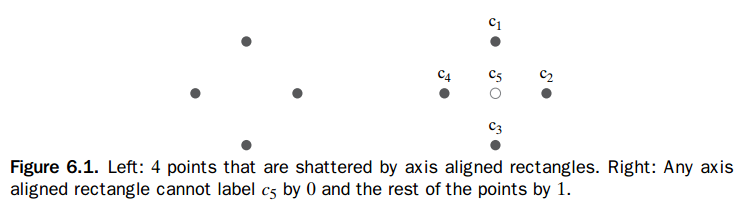
\includegraphics[scale = 0.5]{axis_aligned_rectangle.png}}
\end{minipage}
\caption{\footnotesize{\textbf{(left) There exists a $4$-point set that can be shattered by axis aligned rectangle. (right). Any $5$ point set cannot be shattered.   \citep{shalev2014understanding}}}}
\label{fig: axis_aligned_rectangle}
\end{figure}

\item \begin{example}(\textbf{\emph{Axis Aligned Rectangles}})\\
Let $\cH$ be the class of \emph{\textbf{axis aligned rectangles}}, formally:
\begin{align*}
\cH := \set{h_{(a_1, a_2, b_1, b_2)}: a_1 \le a_2 \land b_1 \le b_2},
\end{align*} where $h_{(a_1, a_2, b_1, b_2)}(x_1, x_2) := \ind{(x_1, x_2) \in [a_1, a_2] \times [b_1, b_2]}$. We shall show in the following that \underline{$\text{VCdim}(\cH) = 4$}.

To prove this we need to \emph{find a set of $4$ points that are shattered by $\cH$}, and show that \emph{\textbf{no set of $5$ points can be shattered by $\cH$}}. Finding a set of $4$ points that are shattered is easy (see Figure \ref{fig: axis_aligned_rectangle}).

Now, consider any set $\cD \subset \bR^2$ of $5$ points. In $\cD$, take a \textit{\textbf{leftmost point}} (whose first coordinate is the smallest in $\cD$), a \emph{\textbf{rightmost point}} (first coordinate is the largest), a \emph{\textbf{lowest point}} (second coordinate is the smallest), and a \emph{\textbf{highest point}} (second coordinate is the largest). Without loss of generality, denote $\cD = \set{x_1 \xdotx{,} x_5}$ and let $x_5$ be the point that \emph{was not selected}. Now, define the labeling $(1,1,1,1,0)$. It is \emph{impossible to obtain this labeling} by an \emph{axis aligned rectangle}. Indeed, such a rectangle must contain $x_1 \xdotx{,} x_4$; but in this case the rectangle contains $x_5$ as well, because its coordinates are within the intervals defined by the selected points. So, $\cD$ is not shattered by $\cH$.
\end{example}



\item \begin{example}(\textbf{\emph{Hyperplanes in $\bR^d$}})\\
Consider the set of \emph{\textbf{hyperplanes}} in $\bR^d$. A hyperplane can be represented as $\inn{w}{x} + b$. Let $\cH$ be set of functions $\sgn{\inn{w}{x} + b}$ for all $w \in \bR^d$ and $b \in \bR$. We claim that \underline{$\text{VCdim}(\cH) = d + 1$}, that is \emph{\textbf{the dimension of parameter set} for hyperplane}.

We derive \emph{a \textbf{lower bound}} by starting with a set of $d + 1$ points in $\bR^d$, setting $x_0$ to be the \emph{origin} and defining $x_i$, for $i \in \set{1 \xdotx{,} d}$, as the point whose $i$-th coordinate is $1$ and all others are $0$. Let $y_0, y_1 \xdotx{,} y_d \in \set{-1,+1}$ be an arbitrary set of labels for $x_0, x_1  \xdotx{,} x_d$. Let $w$ be the vector whose $i$-th coordinate is $y_i$ and $b = y_0/2$. Then the classifier defined by the hyperplane of equation $\inn{w}{x} + y_0/2 = 0$ \emph{shatters}
$x_0, x_1  \xdotx{,} x_d$ since for any $i \in [0, d]$,
\begin{align*}
\sgn{\inn{w}{x_i} +  \frac{y_0}{2}} = \sgn{y_i +  \frac{y_0}{2}} = y_i.
\end{align*}

To obtain \emph{an \textbf{upper bound}}, it suffices to show that \emph{\textbf{no set of $d + 2$ points can be shattered by halfspaces}}. We have the following \emph{\textbf{Radon's theorem}}, which confirms that $\cD$ with $d+2$ points can be \emph{partitioned into two subsets} $\cD_1$ and $\cD_2$ whose \emph{\textbf{convex hull} \textbf{interset}}. Observe that when two sets of points $\cD_1$ and $\cD_2$ are \emph{\textbf{separated by a hyperplane}}, \emph{their convex hulls are also separated by that hyperplane}.  Thus,  $\cD_1$ and $\cD_2$  \emph{\textbf{cannot be separated by a hyperplane}} and $\cD$ is not \emph{shattered}.  Combining our lower and upper bounds, we have proven that the VC-dimenson of hyperplanes in $\bR^d$ is equal to $d+1$.

\begin{theorem} (\textbf{Radon's Theorem}) \citep{mohri2018foundations}\\
Any set $\cX$ of $d+2$ points in $\bR^d$ can be partitioned into two subsets $\cX_1$ and $\cX_2$ such that \textbf{the convex hulls} of $\cX_1$ and $\cX_2$ intersect.
\end{theorem}
\end{example}


\begin{figure}
\begin{minipage}[hb]{1\linewidth}
  \centering
  \centerline{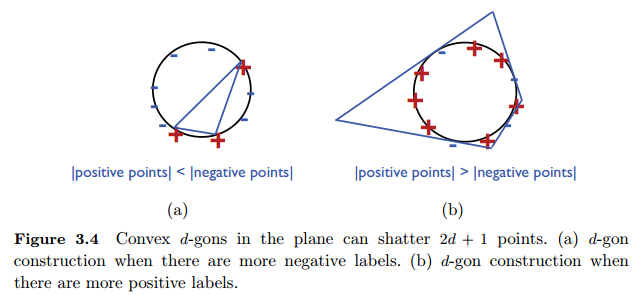
\includegraphics[scale = 0.6]{convex_d_gon_vc_dim.png}}
\end{minipage}
\caption{\footnotesize{\textbf{ Convex d-gons in the plane can shatter $2d + 1$ points. \citep{mohri2018foundations}}}}
\label{fig: convex_d_gon_vc_dim}
\end{figure}



\item \begin{example}(\textbf{\emph{Finite Dimensional Vector Space of Real Functions on $\bR^d$}})\\
Let $\cF$ be a \emph{finite-dimensional vector space} of \emph{real functions} on $\bR^d$, $\text{dim}(\cF) = r < \infty$. Let $\cH$ be the set of
hypotheses,  which we refer to as \emph{\textbf{the subgraph class}} of $\cF$.
\begin{align*}
\cG(\cF) := \set{\set{x \in \bR^d: f(x) \le 0}: f\in \cF}.
\end{align*} We claim that  \underline{$\text{VCdim}(\cG(\cF)) \le r$}.
 (Hint: select an arbitrary set of $m = r + 1$ points and consider linear mapping $u: \cF \to \bR^m$ defined by: $u(f) = (f(x_1) \xdotx{,} f(x_m))$.)
 
We summarize the result in the following proposition
\begin{proposition}(\textbf{Finite-Dimensional Vector Spaces})  \citep{mohri2018foundations, wainwright2019high}\\
Let $\cF$ be a vector space of functions $f: \bR^d \to \bR$ with dimension $\text{dim}(\cF)  = r < \infty$. Then the subgraph class $\cG(\cF)$ has VC
dimension \textbf{at most} $r$.
\end{proposition}
\begin{proof}
Let $x := (x_1 \xdotx{,} x_{m})$ where $m = r + 1$. Consider linear mapping $u_x: \cF \to \bR^m$ induced by $x$ as $u_{x}(f) = (f(x_1) \xdotx{,} f(x_m))$. By construction, the \emph{\textbf{range} of the mapping} $u_x$ is a \emph{linear subspace} of $\bR^m$ with dimension at most $\text{dim}(\cF) = r = m - 1 < m$. Therefore, there must exist a \emph{non-zero vector} $\gamma \in \bR^m$ such that $\inn{\gamma}{u_x(f)} = 0$ for all $f \in  \cF$.  We may assume without loss of generality that at least one coordinate is positive, and then write
\begin{align}
\sum_{i: \gamma_i >0}\gamma_i f(x_i) &= \sum_{j: \gamma_j \le 0}(-\gamma_j) f(x_j), \quad \forall f \in \cF. \label{pf: finite_dim_fun_space_vc_dim}
\end{align} 
Proceeding via proof by \emph{contradiction}, suppose that there were to exist some $f \in  \cF$ such that the associated subgraph set $\set{x \in \bR^d: f(x) \le 0}$ included only the subset samples $\set{x_j:  \gamma_j \le 0}$. For such a function $f$, the left-hand side of equation \eqref{pf: finite_dim_fun_space_vc_dim} would be \emph{strictly positive} while the right-hand side would be \emph{non-positive}, which is a \emph{contradiction}. We conclude that
$\cH(\cF)$ fails to shatter the set $\set{x_1 \xdotx{,} x_{m}}$, as claimed. \qed
\end{proof}
\end{example}



\item \begin{example}(\textbf{\emph{Convex $d$-gons in $\bR^2$}})\\
Consider $\cH$ the class of \textbf{\emph{convex $d$-gons in the plane}}. We claim that \underline{$\text{VCdim}(\cH) = 2d + 1$}, 

To get a lower bound, we show that \emph{\textbf{any set of $2d + 1$ points can be fully shattered}}. To do this, we select $2d + 1$ points that \emph{lie \textbf{on a circle}}, and for a particular labeling, if there are \emph{more negative than positive labels}, then \emph{the \textbf{points} with \textbf{the positive labels} are used as
\textbf{the polygon's vertices}}, as in Figure \ref{fig: convex_d_gon_vc_dim} (a). Otherwise, \emph{the \textbf{tangents} of the \textbf{negative points}} serve as the \emph{\textbf{edges} of the polygon}, as shown in Figure \ref{fig: convex_d_gon_vc_dim} (b).

To derive an upper bound, it can be shown that \emph{choosing \textbf{points on the circle} \textbf{maximizes} \textbf{the number of possible dichotomies}}, and thus $\text{VCdim}(\cH) = 2d + 1$. 

Note also that if $\cH$ is the set of \underline{\emph{\textbf{all convex polygons}}}, then \underline{$\text{VCdim}(\cH) = \infty$}.
\end{example}

\item \begin{example}(\textbf{\emph{Spheres in $\bR^d$}})\\
Consider the space of all $d-1$ dimensional sphere $\cS^{d}$, with sphere $\bS_{a, b} := \set{x \in \bR^d: \norm{x - a}{2} \le b }$. Note that 
\begin{align*}
x \in \bS_{a, b} \Leftrightarrow  f_{a, b}(x) := \norm{x}{2}^2 - 2 \inn{a}{x} +  \norm{a}{2}^2 - b^2 \le 0.
\end{align*} so that the sphere  $\bS_{a,b}$ is a \emph{\textbf{subgraph}} of the function $f_{a,b}$. 

In order to compute the VC dimension of $\cS^{d}$, we first define a feature map $\varphi: \bR^d \to \bR^{d+2}$ via
\begin{align*}
\varphi(x) := (1, x_1 \xdotx{,} x_d, \norm{x}{2}^2)
\end{align*}  and then consider functions of the form
\begin{align*}
g_c(x) := \inn{c}{\varphi(x)}, \quad c\in \bR^{d+2}
\end{align*} The family of functions $\set{g_c, c \in \bR^{d+1}}$ is a vector space of dimension $d + 2$, and it contains the function class $\set{ f_{a,b}, (a, b) \in \bR^d \times \bR_{+}}$. Consequently, by applying Proposition on vector space of real-valued functions  to this larger vector space, we conclude that \underline{$\text{VCdim}(\cS^{d}) \le d+ 2$}. \emph{This bound} is adequate for many purposes, but is \emph{\textbf{not sharp}}: a more careful analysis shows that \underline{\emph{\textbf{the VC dimension} of \textbf{spheres} in $\bR^d$ is actually $d + 1$}}.
\end{example}


\begin{figure}
\begin{minipage}[t]{1\linewidth}
  \centering
  \centerline{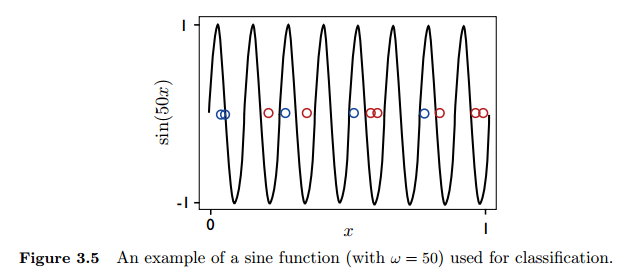
\includegraphics[scale = 0.6]{sine_vc_dim.png}}
\end{minipage}
\caption{\footnotesize{\textbf{The class of sine functions has infinity VC dimension. \citep{mohri2018foundations}}}}
\label{fig: sine_vc_dim}
\end{figure}

\item \begin{example}(\textbf{\emph{Sine Functions}})\\
The previous examples could suggest that \emph{\textbf{the VC-dimension} of $\cH$ coincides with} \emph{\textbf{the number of free parameters} defining $\cH$}.  \underline{\emph{\textbf{However, this does not hold in general}}}. 

The following provides a striking example from this point of view. Consider the following \emph{\textbf{family of sine functions}}: $\cH := \set{t\to \sin(\omega t): \omega \in \bR}$.  One instance of this function class is shown in Figure \ref{fig: sine_vc_dim}. These sine functions can be used to \emph{classify the points on the real line}: a point is labeled \emph{\textbf{positively}} if it is \emph{\textbf{above the curve}}, \emph{negatively} \emph{otherwise}. 

Although this family of sine function is defined via \emph{a single parameter}, $\omega$, it can be shown that \underline{$\text{VCdim}(\cH) = \infty$}.
\end{example}
\end{itemize}

\subsection{Lower Bounds}
\begin{itemize}
\item \begin{remark} (\emph{\textbf{No-Free-Lunch via VC-Dimension}})\\
This section provides \emph{\textbf{lower bounds}} on \emph{the generalization error} of \emph{any learning algorithm} in terms of the \emph{VC-dimension} of the hypothesis set used.

These lower bounds are shown by finding \emph{for any algorithm} a `\emph{\textbf{bad}}' \emph{distribution}. Since the learning algorithm is \emph{arbitrary}, it will be difficult to specify that particular distribution. Instead, it suffices to \emph{prove its \textbf{existence} \textbf{non-constructively}}. At a high level, the proof technique used to achieve this is \emph{\textbf{the probabilistic method}} of Paul Erd\"os. 

In the context of the following proofs, 
\begin{enumerate}
\item \emph{first} \emph{\textbf{a lower bound}} is given on the expected error over \emph{the parameters defining the distributions}.

\item  From that, \emph{the lower bound} is shown to \emph{\textbf{hold for at least one set of parameters}}, that is one distribution.
\end{enumerate}
\end{remark}

\item \begin{proposition} (\textbf{Lower Bound, Realizable Case}) \citep{mohri2018foundations}\\
Let $\cH$ be a hypothesis set with \textbf{VC-dimension} $d > 1$. Then, for \textbf{any} learning algorithm $\cA$, there \textbf{exist} a \textbf{distribution} $\cP$ over $\cX$ and a \textbf{target function} $c \in \cH$ such that
\begin{align*}
\cP^n\set{L_{\cP, c}(\cA_{\cH}(\cD_n)) > \frac{d-1}{32 n}} \ge \frac{1}{100}
\end{align*}
\end{proposition}

\item \begin{remark} (\emph{\textbf{Infinite VC-dimension $\Rightarrow$ Non PAC-learnable}})\\
The theorem shows that for any algorithm $\cA$, there exists a `\emph{bad}' distribution over $\cX$ and a target function $f$ for which the error of the hypothesis returned by $\cA$ is
\begin{align*}
\Omega\paren{\frac{d}{n}}
\end{align*} with some constant probability. This further demonstrates the key role played by the VC-dimension in learning. The result implies in particular that \emph{\textbf{PAC-learning in the non-realizable case} is \textbf{not possible} when the \textbf{VC-dimension} is \textbf{infinite}}.
\end{remark}

\item \begin{proposition} (\textbf{Lower Bound, Non-Realizable Case}) \citep{mohri2018foundations} \\
Let $\cH$ be a hypothesis set with \textbf{VC-dimension} $d > 1$. Then, for any learning algorithm $\cA$, there exists a distribution $\cP$ over $\cX \times \set{0, 1}$ such that:
\begin{align*}
\cP^{n}\set{L_{\cP}(\cA_{\cH}(\cD_n)) - \inf_{h  \in \cH}L_{\cP}(h)  > \sqrt{\frac{d}{320 n}}} \ge \frac{1}{64}
\end{align*} Equivalently, for any learning algorithm, \textbf{the sample complexity} verifies
\begin{align*}
n &\ge \frac{d}{320 \epsilon^2}.
\end{align*}
\end{proposition}

\item \begin{remark}
The theorem shows that \emph{for any algorithm} $\cA$, \emph{\textbf{in the non-realizable case}} (i.e. the Bayes classifier is not in $\cH$), there exists
a `\emph{bad}' distribution over $\cX \times \set{0, 1}$ such that the error of the hypothesis returned by $\cA$ is
\begin{align*}
\Omega\paren{\sqrt{\frac{d}{n}}}
\end{align*} with some constant probability. This coincides with the upper bound $\cO(\sqrt{d/n})$, which means that it is both \emph{necessary and sufficient condition} for PAC learnablity in agnostic setting.

The \emph{VC-dimension} appears as a critical quantity in learning in \emph{this general setting} as well. In particular, \emph{with an \textbf{infinite VC-dimension}, \textbf{agnostic PAC-learning is not possible}}.
\end{remark}
\end{itemize}

\subsection{Fundamental Theorem of PAC Learning}
\begin{itemize}
\item \begin{theorem} (\textbf{The Fundamental Theorem of Statistical Learning}). \citep{shalev2014understanding}\\
Let $\cH$ be a hypothesis class of functions from a domain $\cX$ to $\set{0,1}$ and let the loss function be the $0$-$1$ loss. Then, the following are \textbf{equivalent}:
\begin{enumerate}
\item $\cH$ has the \textbf{uniform convergence property}.
\item Any \textbf{ERM} rule is a successful \textbf{agnostic PAC learner} for $\cH$.
\item $\cH$ is \textbf{agnostic PAC learnable}.
\item $\cH$ is \textbf{PAC learnable}.
\item Any ERM rule is a successful PAC learner for $\cH$.
\item $\cH$ has a \textbf{finite VC-dimension}.
\end{enumerate}
\end{theorem}

\item \begin{remark}
From the above theorem, we see that $\cH$ is \emph{PAC learnable} $\Leftarrow$ $\cH$ is \emph{agnostic PAC learnable}.

If $\cH$ is (agnostic) PAC learnable, then the ERM rule is a successful (agnostic) PAC learner for $\cH$. 
\end{remark}

\item \begin{theorem} (\textbf{The Fundamental Theorem of Statistical Learning, Quantitative Version}). \citep{shalev2014understanding}\\
Let $\cH$ be a hypothesis class of functions from a domain $\cX$ to $\set{0,1}$ and let the loss function be the $0$-$1$ loss. Assume that $\text{VCdim}(\cH) = d < \infty$. Then, there are absolute constants $C_1, C_2$ such that
\begin{enumerate}
\item $\cH$ has the \textbf{uniform convergence property} with sample complexity
\begin{align*}
C_1\frac{d + \log(1/\delta)}{\epsilon^2} \le n^{UC}_{\cH}(\epsilon, \delta) \le C_2\frac{d + \log(1/\delta)}{\epsilon^2}
\end{align*}
\item $\cH$ is \textbf{agnostic PAC learnable} with sample complexity
\begin{align*}
C_1\frac{d + \log(1/\delta)}{\epsilon^2} \le n_{\cH}(\epsilon, \delta) \le C_2\frac{d + \log(1/\delta)}{\epsilon^2}
\end{align*}
\item $\cH$ is \textbf{PAC learnable} with sample complexity
\begin{align*}
C_1\frac{d + \log(1/\delta)}{\epsilon^2} \le n_{\cH}(\epsilon, \delta) \le C_2\frac{d\log(1/\epsilon) + \log(1/\delta)}{\epsilon^2}
\end{align*}
\end{enumerate}
\end{theorem}
\end{itemize}
\newpage
\bibliographystyle{plainnat}
\bibliography{reference.bib}
\end{document}